\section{Introduction} \label{sec:intro}
% What is crossmodal retrieval
Cross-modal retrieval has received a lot of interest in recent years due to the rise of multimodal data. A cross-modal retrieval task is defined as querying an interactive system using one modality and retrieving relevant results from a multimodal database in another modality. A user, for example, can query using text such as "a dog playing with a ball in the garden" and retrieve similar results in other modalities such as images, audio, and video, as shown in Figure\ref{fig:cmr_task}. Effective cross-modal retrieval necessitates bridging the gap between different data modalities, which entails recognizing and localizing objects, determining their attributes, characterizing their relationships, and eventually describing the shared semantic content across multiple modalities.  Thanks to recent advances such as transformer architecture and large pre-trained models, data can be effectively represented as features using domain-specific neural networks. These unimodal features can provide the information required to comprehend multimodal data. A general approach to multi-modal retrieval involves extracting features from individual modalities (image, text, audio, video) and subsequently projecting them onto a common representation space. Within this space, items with similar semantic content exhibit similar representations. Subsequently, a nearest-neighbor search algorithm is used to recommend relevant cross-modal items in this common space.

\begin{figure*}[h]
    \centering
    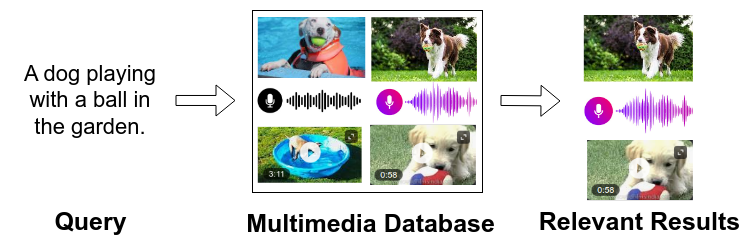
\includegraphics[width=\textwidth]{Figures/task.png}
    \caption{Illustration of Cross-modal Retrieval Task}
    \label{fig:cmr_task}
\end{figure*}

The challenges in developing a cross-modal retrieval system are as follows: 1) We have an enormous amount of multi-modal data available, so an algorithm that is scalable, lightweight, and can train and infer in a reasonable amount of time is required. 2) Different modalities of data follow different distributions when represented using feature embeddings. As a result, there is a heterogeneity gap between the representations of various modalities. Because a cross-modal system can no longer directly compare features from different modalities, an algorithm that can bridge this heterogeneity gap is required. 3) In a supervised setting, each multi-modal item has a single or a set of ground truth labels. If two items share one or more labels, they are semantically nearly or exactly similar, but their feature vectors may differ at the low-level feature level. As a result, an algorithm that can handle multiple labels, correlate them, and bridge the gap between high-level semantics and low-level features is required. 4) In the real world, data from various modalities may arrive at different times. As a result, an algorithm capable of adding new modality data in parallel or after training existing modalities is required. 5) Once the system has learned a compact common representation for multi-modal data and the query, an efficient indexing and nearest neighbor search algorithm that can effectively utilize the learned common representation is required. 

Similar to the cross-modal retrieval task, the task of evaluating cross-modal generative models is also very challenging. A cross-modal generative task is defined as generating new data in one modality (e.g., text, images) based on input data in another modality. A user, for example, can ask for an image of "A dog playing with a ball in the garden." and get a generated result, as shown in Figure\ref{fig:gen}. Traditional heuristic-driven evaluation metrics for generative models often fall short in terms of usability and interpretability, especially when dealing with the increasingly creative and nuanced outputs of recent LLM-based and diffusion-based models. Thus, a new framework capable of providing usability and interpretability is required. 

\begin{figure*}[h]
    \centering
    \includegraphics[width=\textwidth]{Figures/gen.png}
    \caption{Example of Cross-modal Generative Task}
    \label{fig:gen}
\end{figure*}

\par Traditional cross-modal retrieval methods \cite{ocmfh, lsrh} use linear projection matrix to project the features into the common space, while other methods tend to use kernel operations \cite{srlch, dch} to account for non-linearity in the multi-modal data. To account for storage and computation costs, hashing methods have recently gained much attention. These methods aim to learn low-dimensional binary codes for high-dimensional input features such that the binary codes preserve inter- and intra-modal similarity. Recent cross-modal retrieval methods either use deep cross-modal neural networks \cite{dsmhn,acmr,sdml,dvsh} or multimodal transformer architecture \cite{BLIP, VILT} to learn the mapping between multi-modal data. There are four challenges that the prior work has paid little attention to. 1) Most real-valued and deep cross-modal retrieval methods do not account for learning a scalable and lightweight transformation of feature embeddings into a common space. 2) Most supervised cross-modal retrieval methods except \cite{ssah,svhn} do not ensure that the nearly similar items have similar common representations. 3) Almost all cross-modal retrieval methods except \cite{sdml, svhn, joint} do not ensure adding new modalities of data without learning the common representation space from scratch. 4) Almost all cross-modal methods except \cite{jgrhml,cdpae} use the exhaustive search algorithm to recommend relevant items for the query without considering the learned characteristics of the common space. Similarly, the existing heuristic-driven evaluation metrics for cross-modal generative models like BLEU Score \cite{bleu}, FID \cite{FID}, BERTScore \cite{BERTScore}, CLIPScore \cite{CLIPScore}, etc. are not easily interpretable. Their scores are not robust to changes like using synonyms, adding or removing stopwords, color conversions in images, etc. 

In this thesis, we propose a novel cross-modal retrieval framework called LCM and its extension, LM-I to address the aforementioned challenges in the cross-modal retrieval literature. To address the difficulties in evaluating cross-modal generative models, we propose a novel cross-modal retrieval framework that compares various generative models using existing information retrieval metrics such as Normalised Discounted Cumulative Gain (nDCG\textquotesingle@K) and Ranked Biased Precision (RBP\textquotesingle@K). The contributions of this thesis can be summarized as follows:
\begin{itemize}
    \item We propose a scalable and lightweight cross-modal retrieval method that can adapt to any new modality, such as audio, in addition to image and text.
    \item We propose a unified cross-modal retrieval framework that uses generative augmentation for the retrieval task to evaluate cross-modal generative models.
\end{itemize}

% % Applications of cross-modal retrieval
% Cross-modal retrieval is not only useful for searching tasks like finding a relevant description of an image or finding the movie trailer given the movie's description, but it can also be useful in evaluating foundational models to determine whether they have learned the alignment of different data modalities. Vision-language foundational models today are responsible for solving numerous tasks like visual question answering, image captioning, image generation, image retrieval, text retrieval, etc. The effectiveness of solving these tasks evaluates the learned representations of the foundational models. Thus, the retrieval task can be important in evaluating cross-modal generative models like image captioning and image generation models.